%%%%%%%%%%%%%%%%%%%%%%%%%%%%%%%%%%%%%%%%%%%%%%%%%%%%%%%%%%%%%%%%%%%
%                                                                 %
%   HBOOK - Reference Manual -- LaTeX Source                      %
%                                                                 %
%   Front Material: Title page,                                   %
%                   Copyright Notice                              %
%                   Preliminary Remarks                           %
%                   Table of Contents                             %
%   EPS file      : cern15.eps, cnastit.eps                       %
%                                                                 %
%   Editor: Michel Goossens / CN-AS                               %
%   Last Mod.:  9 December 1993 11:40 mg                          %
%                                                                 %
%%%%%%%%%%%%%%%%%%%%%%%%%%%%%%%%%%%%%%%%%%%%%%%%%%%%%%%%%%%%%%%%%%%

%%%%%%%%%%%%%%%%%%%%%%%%%%%%%%%%%%%%%%%%%%%%%%%%%%%%%%%%%%%%%%%%%%%%
%    Tile page                                                     %
%%%%%%%%%%%%%%%%%%%%%%%%%%%%%%%%%%%%%%%%%%%%%%%%%%%%%%%%%%%%%%%%%%%%
%begin{latexonly}
\def\Ptitle#1{\special{ps: /Printstring (#1) def}
                       \epsfbox{../cnasall/cnastit.eps}}
\begin{titlepage}
\vspace*{-23mm}
\includegraphics[height=30mm]{cern15.eps}%
\hfill
\raisebox{8mm}{\Large\bf CERN Program Library Long Writeups Y250}
\hfill\mbox{}
\begin{center}
\mbox{}\\[10mm]
\mbox{\Ptitle{HBOOK}}\\[2cm]
{\Huge Statistical Analysis and Histogramming}\\[2cm]
{\Huge Reference Manual}\\[5cm]
{\Large Information Technology Division}\\[2cm]
\end{center}
\begin{center}\Large CERN Geneva, Switzerland\end{center}
\end{titlepage}
%end{latexonly}
\begin{htmlonly}
\begin{center}{\Large\bf CERN Program Library Long Writeup D506}\\[1cm]
{\Huge HBOOK}\\[2cm]
{\Huge Statistical Analysis and Histogramming}\\[2cm]
{\Huge Reference Manual}\\[5cm]
{\Large Information Technology Division}\\[2cm]
{\Large CERN Geneva, Switzerland}
\end{center}

\begin{rawhtml}
<HR>
<H3><A href="http://wwwinfo.cern.ch/asd/cernlib/hbook/hbook.ps">
PostScript version of this manual</A></H3>
<HR>
\end{rawhtml}
\end{htmlonly}


%%%%%%%%%%%%%%%%%%%%%%%%%%%%%%%%%%%%%%%%%%%%%%%%%%%%%%%%%%%%%%%%%%%%
%    Copyright  page                                               %
%%%%%%%%%%%%%%%%%%%%%%%%%%%%%%%%%%%%%%%%%%%%%%%%%%%%%%%%%%%%%%%%%%%%
\begin{htmlonly}
\chapter{Copyright Notice}
\end{htmlonly}
%begin{latexonly}
\thispagestyle{empty}
\framebox[\textwidth][t]{\hfill\begin{minipage}{0.96\textwidth}%
\vspace*{3mm}
\begin{center}Copyright Notice\end{center}
\parskip\baselineskip
%end{latexonly}
{\bf HBOOK -- Statistical Analysis and Histogramming}
 
CERN Program Library entry {\bf Y250}
 
\copyright{} Copyright CERN, Geneva 1995--1998
 
Copyright and any other appropriate legal protection of these
computer programs and associated documentation reserved in all
countries of the world.
 
These programs or documentation may not be reproduced by any
method without prior written consent of the Director-General
of CERN or his delegate.
 
Permission for the usage of any programs described herein is
granted apriori to those scientific institutes associated with
the CERN experimental program or with whom CERN has concluded
a scientific collaboration agreement.
 
Requests for information should be addressed to:
%begin{latexonly}
\vspace*{-.5\baselineskip}
\begin{center}
\tt\begin{tabular}{l}
CERN Program Library Office              \\
CERN-IT Division                         \\
CH-1211 Geneva 23                        \\
Switzerland                              \\
Tel.   +41 22 767 4951                   \\
Fax.   +41 22 767 8630                   \\
Email: cernlib@cern.ch
\end{tabular}
\end{center}
\vspace*{2mm}
\end{minipage}\hfill}%end of minipage in framebox
\vspace{6mm}
%end{latexonly}
\begin{htmlonly}
\begin{flushleft}
CERN Program Library Office              \\
CERN-IT Division                         \\
CH-1211 Geneva 23                        \\
Switzerland                              \\
Tel.: +41 22 767 4951                    \\
Fax.: +41 22 767 8630                    \\
Internet: \texttt{cernlib@cern.ch}                
\end{flushleft}
\end{htmlonly}
 
%begin{latexonly}
{\bf Trademark notice: All trademarks appearing in this guide are acknowledged as such.}
\vfill
\begin{tabular}{l@{\quad}l@{\quad}>{\tt}l}
{\em Contact Person\/}:        & Olivier Couet /IT   & (couet@cern.ch)\\[1mm]
{\em Technical Realization\/}: & Michel Goossens /IT & (goossens@cern.ch)\\[1cm]
{\em Edition -- August 1998}
\end{tabular}
%end{latexonly}
\begin{htmlonly}
{\bf Trademark notice: All trademarks appearing in this guide are acknowledged as such.}

\begin{tabular}{lll}
\emph{Contact Person}:           & Olivier Couet /IT   & \texttt{couet@cern.ch}\\
\emph{Documentation consultant}: & Michel Goossens /IT & \texttt{goossens@cern.ch}\\
\emph{Edition -- August 1998}
\end{tabular}
\end{htmlonly}
\newpage
 
%%%%%%%%%%%%%%%%%%%%%%%%%%%%%%%%%%%%%%%%%%%%%%%%%%%%%%%%%%%%%%%%%%%%
%    Introductory material                                         %
%%%%%%%%%%%%%%%%%%%%%%%%%%%%%%%%%%%%%%%%%%%%%%%%%%%%%%%%%%%%%%%%%%%%
%begin{latexonly}
\pagenumbering{roman}
\setcounter{page}{1}

\chapter*{Foreword}

\section*{History}
%end{latexonly}
\begin{htmlonly}
\chapter{Foreword}
\subsection*{History}
\end{htmlonly}

HBOOK is a Fortran\footnote{A C interface is also distributed by
the CERN Program Library, created using the tool f2h} callable 
package for histogramming and fitting.
It was originally developed in the 1970s and has since
undergone continuous evolution culminating
in the current version, HBOOK~4.
 
Many people have contributed to the design and development of HBOOK,
through discussions, comments and suggestions.
 
For many years and up to November 1994 Ren\'e Brun 
has been responsible for the HBOOK program.
Paolo Palazzi was involved in the original design.
D.~Lienart has been in charge of the parametrization part. 
Fred~James is the author of routine \Rind{HDIFF} and of the minimization
package Minuit, which forms the basis of the fitting routines.
The idea of Profile histograms has been taken from the HYDRA system.
The Column-wise-Ntuple routines were implemented by Fons Rademakers.
The multi-dimensional quadratic fit package \Rind{HQUAD} is the work of
John Allison.
J.~Linnemann and his colleagues of the D0 experiment contributed
the routine \Rind{HDIFFB}.
Pierre Aubert is the author of the routines to associate labels
with histograms.
Roger Barlow and Christine Beeston (OPAL) have developed the 
\Rind{HMCMLL} package.
Julian Bunn is the author of the \Rind{HNFORM} routine.


%begin{latexonly}
\section*{Preliminary remarks}
%end{latexonly}
\begin{htmlonly}
\subsection*{Conventions}
\end{htmlonly}
 
This manual serves at the same time as a {\bf Reference manual}
and as a {\bf User Guide} for the HBOOK system.
After a short introductory chapter, where the basic ideas
are explained, the following chapters describe in detail
the calling sequences for the different user routines.
 
In this test examples are in {\tt monotype face} and strings to be
input by the user are {\tt\underline{underlined}}.  In the index the
page where a routine is defined is in {\bf bold}, page numbers where a
routine is referenced are in normal type.

In the description of the routines a \Lit{*} following
the name of a parameter indicates that this is an {\bf output} parameter.
If another \Lit{*} precedes a parameter in the calling sequence, the
parameter in question is both an {\bf input} and {\bf output} parameter.

Some informations about HBOOK can also be found on the Web in the ``PAW
frequently asked questions'' page
\begin{verbatim}
                      http://wwwinfo.cern.ch/asdcgi/listpawfaqs.pl
\end{verbatim}

%begin{latexonly}

This document has been produced using \LaTeX~\cite{bib-LATEX}
with the \Lit{cernman} style option, developed at CERN. 

%%%%%%%%%%%%%%%%%%%%%%%%%%%%%%%%%%%%%%%%%%%%%%%%%%%%%%%%%%%%%%%%%%%%
%    Tables of contents ...                                        %
%%%%%%%%%%%%%%%%%%%%%%%%%%%%%%%%%%%%%%%%%%%%%%%%%%%%%%%%%%%%%%%%%%%%
\newpage
\tableofcontents
\listoffigures
\listoftables
\cleardoublepage
%end{latexonly}

